\usetikzlibrary{arrows.meta}
\tikzset{%
  >={Latex[width=2mm,length=2mm]},
  % Specifications for style of nodes:
            minerbase/.style = {rectangle,
                           minimum width=3cm, minimum height=1cm,
                           text centered, font=\stfamily},
            base/.style = {rectangle, rounded corners, draw=black,
                           minimum width=3cm, minimum height=1cm,
                           text centered, font=\sffamily},
  censoredminer/.style = {minerbase, draw=red!30},
  uncensoredminer/.style = {minerbase, draw=blue!30},
  majority/.style = {base, fill=blue!30},
  minority/.style = {base, fill=red!30},
    common/.style = {base, fill=green!30},
 blacklist/.style = {base, minimum width=2cm, fill=orange!70}
}

\subsection{Expected Results}
In addition to designing experiments to test how the bitcoind client behaves, we also analyzed its source code. According to the source code, if a client is told that a block exists, but is unable to get a copy of that block and validate it, the client will continue assuming the last head of the blockchain it validated is the current head\footnote{Specifically, line 2668 validation.cpp in bitcoind version 0.14: https://github.com/bitcoin/bitcoin/blob/0.14/src/validation.cpp#L2668}. In the scenario we consider, the censored client would be able to recieve a message from non-censored clients telling it that a new block exists. But when the client then requested the contents of the block from the non-censored clients, the respone containing the new block's data would would never be recieved. From the point of view of the censored client, this is indistingushable from a miner broadcasting headers but not sending the full block data. The source code for bitcoind explicitly describes such an attack and contains logic to ensure, in this scenario, the block is not added to a client's index.

\begin{figure}[h]
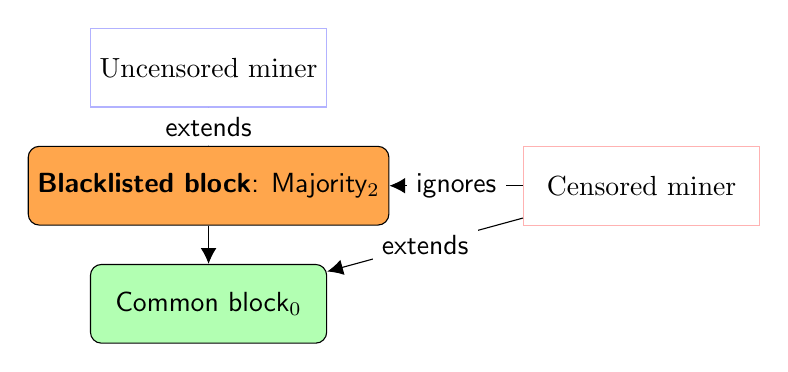
\begin{tikzpicture}[every node/.style={node distance=1.5cm,fill=white, font=\sffamily}, align=center]
  %\node (majority2)[majority, above of=majority1] {Majority block};
  \node (bad)   [blacklist]                {\textbf{Blacklisted block}: Majority$_2$};

  \node (fmine)[uncensoredminer, above of=bad] {Uncensored miner};
  \node (cmine)[censoredminer, right of=bad, xshift=4cm] {Censored miner};
  \node (start)  [common, below of=bad]    {Common block$_0$};

    \draw[->]             (bad) -- (start);
    \draw[->]             (fmine) -- node{extends} (bad);
    \draw[->]             (cmine) -- node{extends} (start);
    \draw[->]             (cmine) -- node{ignores} (bad);
\end{tikzpicture}
\caption{Expected results immediately after a censored block is mined}
\end{figure}

\begin{figure}[h]
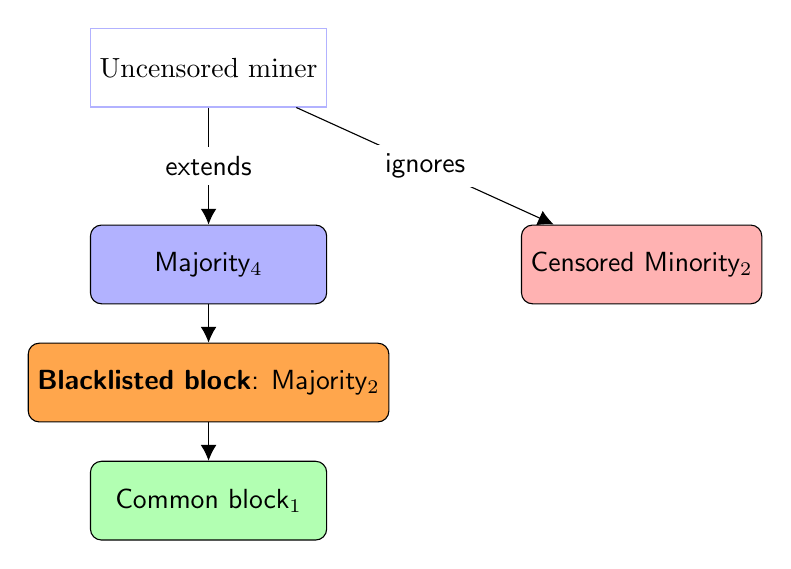
\begin{tikzpicture}[every node/.style={node distance=1.5cm,fill=white, font=\sffamily}, align=center]
  %\node (majority2)[majority, above of=majority1] {Majority block};

  \node (bad)   [blacklist]                {\textbf{Blacklisted block}: Majority$_2$};
  \node (start)  [common, below of=bad]    {Common block$_1$};
  \node (majority1)[majority, above of=bad] {Majority$_4$};
  \node (miner)[uncensoredminer, above of=majority1, yshift=1cm] {Uncensored miner};
  \node (minority)[minority, right of=majority1, xshift=4cm] {Censored Minority$_2$};

    \draw[->]             (miner) -- node{ignores} (minority);
    \draw[->]             (miner) -- node{extends} (majority1);
    \draw[->]             (majority1) -- (bad);
    \draw[->]             (bad) -- (start);
\end{tikzpicture}
\caption{Expected results when a minority is censored, from the perspective of an uncensored minor}
\end{figure}
